\documentclass[aspectratio=169]{beamer}
\usetheme{Madrid}
\usecolortheme{beaver}
\usepackage[utf8]{inputenc}
\usepackage[T1]{fontenc}
\usepackage{tikz}
\usepackage{amssymb}
\usepackage{graphicx}
\setbeamertemplate{navigation symbols}{}
\setbeamercolor{title}{fg=white,bg=cyan!60!black}
\setbeamercolor{frametitle}{fg=white,bg=cyan!50!black}
\setbeamercolor{block title}{bg=cyan!15,fg=black}
\setbeamercolor{block body}{bg=cyan!5,fg=black}

\title{G1 — Sprite Start}
\subtitle{Lesson 2: Four Corners}
\author{ByteForge --- Grade 7 --- Game Maker}
\date{}

\begin{document}

\begin{frame}
    \titlepage
\end{frame}

\begin{frame}{Reading coordinates precisely}
    \Large
    "Draw 4 things" and "draw 4 things in specific places" are very different tasks — real challenges almost always care about WHERE, not just how many.

    \begin{center}
    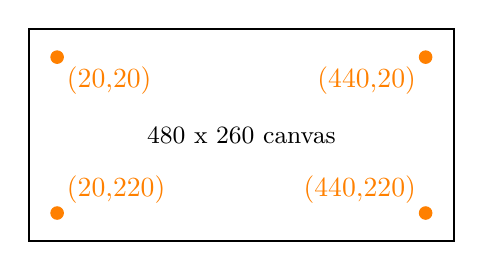
\begin{tikzpicture}[scale=0.9]

        \draw[thick] (0,0) rectangle (6,-3);
        \filldraw[orange] (0.4,-0.4) circle (2.5pt) node[below right] {(20,20)};
        \filldraw[orange] (5.6,-0.4) circle (2.5pt) node[below left] {(440,20)};
        \filldraw[orange] (0.4,-2.6) circle (2.5pt) node[above right] {(20,220)};
        \filldraw[orange] (5.6,-2.6) circle (2.5pt) node[above left] {(440,220)};
        \node at (3,-1.5) {\small 480 x 260 canvas};
    \end{tikzpicture}
    \end{center}
\end{frame}

\begin{frame}{Reading coordinates precisely --- Worked Example}
    \Large
    Worked example: "top-left" isn't (0,0) exactly — it's (20,20), a small margin in from the true edge, so a sprite isn't drawn half off-screen.
\end{frame}

\begin{frame}{Your Turn}
    \Large
    Open the student map, find \textbf{G1 — Sprite Start}, and complete
    the \textbf{Four Corners} challenge --- everything you just saw, they now do themselves.
\end{frame}

\end{document}
